\documentclass[11pt,a4paper]{article}

\usepackage[margin=1in]{geometry}
\usepackage{amsmath,amssymb}
\usepackage{graphicx}
\usepackage{hyperref}
\usepackage{enumitem}

\setcounter{secnumdepth}{2}

\title{Research proposal:Testing a spectral epidemic threshold for SIS on networks under heavy-tailed recovery}
\author{} % optional
\date{} % optional

\begin{document}
\maketitle

\begin{abstract}
Many infectious diseases do not give permanent immunity: people can be infected, recover, and then become infected again. A key practical question is when an introduced infection will quickly disappear from a population and when it can keep circulating at a low but persistent level. Simple mathematical models often use a compact rule of thumb to decide whether an infection is ``under control'', based on how easily it spreads, how long people stay infectious on average, and how well the population is connected. In reality, however, recovery times are very irregular. In this project we use an agent-based computer simulation of an infection spreading through a network of individuals to test how robust such simple threshold rules are when recovery times have long tails. We compare scenarios with ``regular'' recovery times to scenarios with strongly varying, heavy-tailed recovery, while keeping the mean recovery time the same. Our hypothesis is that heavy-tailed recovery will make it easier for the infection to persist than the standard rule of thumb would suggest, even when the average recovery time is unchanged.
\end{abstract}

\section{Background}

Many real-world infections do not give permanent immunity. People can be infected, recover, and then become infected again, sometimes multiple times in their life. Examples include common colds, certain sexually transmitted infections, and hospital-acquired infections. A central practical question is: \emph{when does an introduced infection die out quickly, and when can it keep circulating in a population for a long time?} This boundary between die-out and long-term persistence is often called the epidemic (or endemic) threshold.

In a basic SIS (susceptible--infected--susceptible) model on a network, each individual is either healthy and susceptible or currently infected, and recovery is typically assumed to follow a simple, memoryless process. A standard summary of how easily infection can take hold is an \emph{effective transmission} intensity $\tau$ that combines per-contact infection strength with the mean infectious period. Spectral arguments then predict an epidemic (endemic) threshold of the form
\[
  \tau_c \approx \frac{c}{\lambda_{\max}},
\]
where $\lambda_{\max}$ is the largest eigenvalue of the adjacency matrix and $c$ is a constant. In a homogeneous mean-field limit one often takes $c=1$; on a finite network, in discrete time, and with correlations beyond mean field, the effective $c$ need not be exactly one, but the scaling with $1/\lambda_{\max}$ remains the usual reference. Equivalently, at fixed mean recovery time $\mathbb{E}[W]$, the implied critical \emph{infection probability} is $\beta_c \approx \tau_c/\mathbb{E}[W] \approx c/(\lambda_{\max}\mathbb{E}[W])$. This spectral picture has been widely used and analysed in network epidemiology (\ Chakrabarti et al.\ 2008; Van Mieghem 2011; Pastor-Satorras et al.\ 2015).

However, real recovery times are often far from this idealised picture. Tang et al.\ (2025) introduce the grp-SIS framework as a generalisation of the basic SIS model, allowing more flexible recovery-time patterns for infected individuals, including heavy-tailed distributions, while keeping the same basic SIS structure of possible reinfection. Together with other work on SIS models with general or heavy-tailed recovery (e.g.\ Cator et al.\ 2013), this confirms that the \emph{shape} of the recovery-time distribution can strongly influence dynamics, even when the \emph{mean} recovery time is kept fixed.

What is much less clear from existing theory is whether the simple scaling $\tau_c \approx c/\lambda_{\max}$ (and the mean-field benchmark $c=1$) still describes the threshold well once we move away from exponential recovery towards more realistic, heavy-tailed recovery times. This question matters for practice because such rules of thumb are sometimes used to judge whether an infection is ``under control'' on a given contact structure. Agent-based modelling (ABM) offers a natural way to explore this gap: by simulating many individuals on an explicit contact network, with realistic recovery-time distributions, we can directly observe whether infections die out or persist under different parameter settings, without relying only on mean-field approximations (i.e., replacing detailed neighbour-to-neighbour correlations with average infection levels in the population).

In this project we therefore use a NetLogo agent-based SIS model on a simple random network (Erd\H{o}s--R\'enyi~\cite{ErdosRenyi1959} with about 2000 nodes and average degree around 6) as a numerical ``laboratory'' (see Figure~\ref{fig:er-network} for an example network). 


\begin{figure}[tbp]
  \centering
  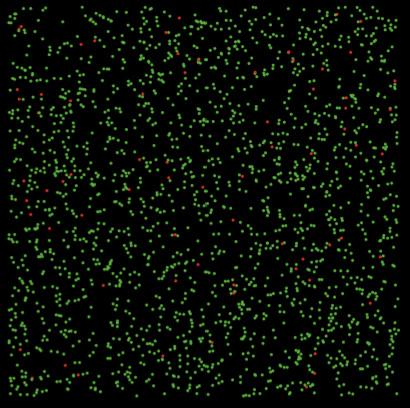
\includegraphics[width=0.6\textwidth]{er_network_example.png}
  \caption{Example of an Erd\H{o}s--R\'enyi~\cite{ErdosRenyi1959} contact network with about 2000 nodes and average degree around 6, as used in the agent-based simulations. Red individuals represent infected agents; other individuals are susceptible.}
  \label{fig:er-network}
\end{figure}

Within this setting we compare exponential (Markovian) recovery to heavy-tailed power-law and lognormal recovery, while keeping the mean recovery time $\mathbb{E}[W]$ fixed. This allows us to test how robust the spectral scaling $\tau_c \approx c/\lambda_{\max}$ remains in an explicit agent-based model and to see whether heavy-tailed recovery mainly shifts the epidemic threshold or primarily affects extinction times and variability.


\section{Research question}

Our hypothesis is that heavy-tailed recovery makes it easier for the infection to persist in the population than a simple spectral threshold rule would suggest, even when the mean recovery time $\mathbb{E}[W]$ is held fixed. In other words, persistence may set in at a lower effective $\tau$ than the mean-field line $\tau_c \approx 1/\lambda_{\max}$ (i.e.\ $c=1$) would suggest, once recovery times are allowed to have long tails.

We address the following research questions to test this hypothesis in the agent-based model on Erd\H{o}s--R\'enyi networks with fixed parameters (about 2000 nodes and average degree around 6):

\begin{itemize}[leftmargin=*]
  \item \textbf{RQ1}.To what extent does the empirically observed threshold---in \emph{infection probability} or in $\tau$ (\emph{infection probability}$\times$\emph{mean recovery time})---agree with the spectral reference $\tau_c \approx c/\lambda_{\max}$ under the mean-field benchmark $c=1$, for an exponential (Markovian) recovery distribution?
  \item \textbf{RQ2}. How does the empirical threshold shift when the recovery distribution is replaced by Tang et al.'s power law or lognormal recovery, while keeping $\mathbb{E}[W]$ fixed?
  \item \textbf{RQ3}. On this Erd\H{o}s--R\'enyi topology (fixed \emph{number of nodes} and \emph{average degree}), does heavy-tailed recovery (power law or lognormal) lead to a systematically different empirical threshold (in terms of infection probability) compared to exponential recovery, or are differences mainly visible in extinction-time distributions and prevalence variability?
\end{itemize}

\section{Research method}
\label{sec:research-method}

\subsection*{Problem and research questions}

The study tests the hypothesis and \textbf{RQ1}-\textbf{RQ3} stated in Section~2: whether simple threshold ideas still match simulation outcomes when recovery times are allowed to be long-tailed, while the mean recovery time is unchanged. The focus is on a \emph{fixed} Erd\H{o}s--R\'enyi \emph{specification} (same \emph{number of nodes} and \emph{average degree}), so differences come primarily from recovery patterns on one graph draw.

\subsection*{Research setup}

\begin{itemize}[leftmargin=*]
  \item \textbf{Simulated world}. Individuals are nodes on an Erd\H{o}s--R\'enyi graph~\cite{ErdosRenyi1959} generated in NetLogo with about \emph{number of nodes}${}=2000$ and \emph{average degree}${}=6$. 

  \item \textbf{Infection process}. A standard agent-based SIS process runs on each such network: infection can spread along links; after recovery an individual can be infected again. The NetLogo model sets \emph{infection probability} (strength of transmission per time step along a link).

  \item \textbf{What we vary}. (i)~The infection strength \emph{infection probability}, swept over many values. (ii)~The recovery time pattern: first a simple ``memoryless'' exponential pattern, then two heavy-tailed options implemented as in Tang et al.\ (power law and lognormal).

  \item \textbf{What we keep fixed}. The graph, the generative specification (topology \emph{number of nodes}, \emph{average degree}), and the \emph{mean recovery time}, so comparisons between recovery regimes are fair at the same $\mathbb{E}[W]$.

  \item \textbf{Reference prediction from the network}. The contact list is exported to a CSV file. In Python, we compute the largest eigenvalue $\lambda_{\max}$ of the adjacency matrix. The mean-field spectral reference is $\tau_c \approx 1/\lambda_{\max}$ (i.e.\ $c=1$ in $\tau_c \approx c/\lambda_{\max}$). At fixed mean recovery time $\mathbb{E}[W]$, the corresponding critical \emph{infection probability} is $\beta_c \approx 1/(\lambda_{\max}\,\mathbb{E}[W])$, which is what sweeps compare against on the probability axis.
\end{itemize}

\subsection*{Measurement and comparison}

\begin{itemize}[leftmargin=*]
  \item \textbf{What we log each run}. Whether the infection died out before the time limit; if so, how long that took; if not, the average share of infected individuals in a late time window.

  \item \textbf{Empirical threshold}. For each recovery pattern, we estimate the smallest \emph{infection probability} at which the infection \emph{typically} stays present (many repeated runs), translate to $\tau$ via \emph{infection probability}$\times$\emph{mean recovery time}, and compare to $\tau_c \approx 1/\lambda_{\max}$ and to the exponential case.

  \item \textbf{Effective transmission}. The scale $\tau$ given by \emph{infection probability}$\times$\emph{mean recovery time} is the simulation counterpart to the $\tau$ in $\tau_c \approx c/\lambda_{\max}$.

  \item \textbf{Link to RQ1--RQ3}. \textbf{RQ1}: agreement between the empirical threshold and the mean-field line $\tau_c \approx 1/\lambda_{\max}$ under exponential recovery. \textbf{RQ2}: how the empirical threshold moves under Tang power-law and lognormal recovery at fixed mean recovery time. \textbf{RQ3}: whether mismatches show up mainly as a different threshold location or mainly as different extinction times and variability in prevalence, even when threshold estimates are similar.
\end{itemize}

\subsection*{Execution}

\begin{itemize}[leftmargin=*]
  \item Build the ER network in NetLogo, export links, compute $\lambda_{\max}$ in Python.
  \item Run NetLogo simulations over \emph{infection probability} on a fine grid around the predicted threshold: exponential recovery first, then power law, then lognormal, with the same sweep range and repetition count. Then run a Python pipeline to merge outputs.
\end{itemize}

\subsection*{Data analysis}

Plot persistence (or late-window prevalence) against \emph{infection probability} (or against $\tau$) for all three recovery types; mark the mean-field reference $\tau_c \approx 1/\lambda_{\max}$ and the implied $\beta_c \approx 1/(\lambda_{\max}\mathbb{E}[W])$ on the probability axis. Compare estimated thresholds and, for \textbf{RQ3}, contrast distributions of extinction times and variability in outcomes. Interpret results against the hypothesis and the literature on spectral threshold rules and non-Markovian recovery.

\section{Time schedule (10 weeks)}

The schedule mirrors Section~\ref{sec:research-method} (Research method). Weeks~1--2 cover Problem and research questions and Research setup, including the NetLogo agent-based model. Weeks~3--6 follow \textbf{RQ1} Execution (week~3), \textbf{RQ2} Execution (week~4), \textbf{RQ3} Execution (week~5), then Measurement and comparison (week~6). Week~7 is Data analysis. Weeks~8--10 deliver the written report and freeze the NetLogo model, experiments, and exported data as reproducible artifacts.

\section{Risk analysis}

\subsection*{Mismatch between discrete simulation and continuous-time theory}

The mean-field reference $\tau_c \approx 1/\lambda_{\max}$ (and the implied $\beta_c$ on the infection-probability axis) is tied to a continuous-time Markovian (exponential recovery) idealisation, whereas the NetLogo model is discrete-time with per-tick probabilities, which may cause systematic differences; for heavy-tailed recovery the same spectral line is used only as a \emph{benchmark}, not as a formally derived grp-SIS threshold. This can make empirical thresholds hard to match to the reference, with deviations that are partly numerical and partly conceptual (non-Markovian recovery). Mitigation: keep per-tick probabilities in a range where a Poisson-style interpretation is plausible; emphasise relative shifts between recovery regimes on the same network; treat absolute agreement with $\tau_c \approx 1/\lambda_{\max}$ mainly as a check for the exponential case (\textbf{RQ1}).

\subsection*{Complexity of BehaviorSpace experiments and data volume}

Pre-defined experiments still imply many runs when combining broad \emph{infection\-probability} sweeps, several recovery distributions, and repetitions, so exports can be large and time pressure within the 10-week window is real. Mitigation: the XML already structures sweeps and metrics; add coarse-to-fine exploration where needed, automated analysis (\texttt{scripts/}), a clear \texttt{output/} layout, disk monitoring, and prioritise runs that map to \textbf{RQ1--RQ3}.

\subsection*{Interpretation under strong stochasticity}

Around the threshold and with heavy-tailed recovery, run-to-run variability may be large, complicating threshold estimation and leaving small shifts in the threshold uncertain. Mitigation: many repetitions per parameter setting and confidence intervals; quasi-stationary analysis (conditioning on non-extinct runs) to estimate steady-state properties.

\begin{thebibliography}{99}

\bibitem{ErdosRenyi1959}
P.~Erd\H{o}s and A.~R\'enyi.
\newblock On random graphs.
\newblock \emph{Publ.\ Math.\ Debrecen} 6, 290--297 (1959).

\bibitem{Cator2013}
E.~Cator, R.~van de Bovenkamp, and P.~Van Mieghem.
\newblock Susceptible--infected--susceptible epidemics on networks with general infection and cure times.
\newblock \emph{Phys.\ Rev.\ E} 87, 062816 (2013).

\bibitem{Chakrabarti2008}
D.~Chakrabarti, Y.~Wang, C.~Wang, J.~Leskovec, and C.~Faloutsos.
\newblock Epidemic thresholds in real networks.
\newblock \emph{ACM Trans.\ Inf.\ Syst.\ Secur.} 10, 13 (2008).

\bibitem{PastorSatorras2015}
R.~Pastor-Satorras, C.~Castellano, P.~Van Mieghem, and A.~Vespignani.
\newblock Epidemic processes in complex networks.
\newblock \emph{Rev.\ Mod.\ Phys.} 87, 925--979 (2015).

\bibitem{Tang2025}
J.~Tang, Y.~Yao, M.~Xie, and M.~Feng.
\newblock SIS epidemic modelling on homogeneous networked system: General recovering process and mean-field perspective.
\newblock \emph{Appl.\ Math.\ Modelling} (2025); preprint arXiv:2505.12290v2.

\bibitem{VanMieghem2011}
P.~Van Mieghem.
\newblock The $N$-intertwined SIS epidemic network model.
\newblock \emph{Computing} 93, 147--169 (2011).

\end{thebibliography}

\end{document}
